\documentclass[12pt]{amsart}
\usepackage[pdftex,colorlinks,citecolor=blue,urlcolor=blue]{hyperref}
\usepackage{amssymb}
\usepackage{graphicx,color}
\usepackage{tikz}
\usepackage{amsmath}

\begin{document}

  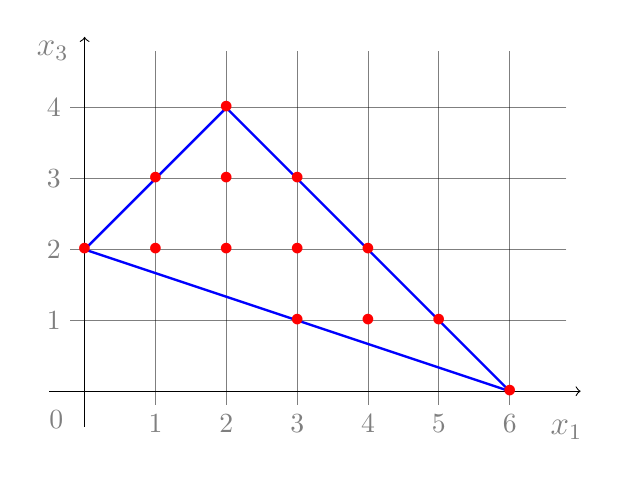
\begin{tikzpicture}[xscale=0.09,yscale=0.09,domain=0.125:220,samples=400]
    \node[opacity=0.5] at (-4,-4) {$0$};

    \draw[->] (-5,0) -- (70,0) node[below] {};
    \draw[->] (0,-5) -- (0,50) node[left] {};
    \foreach \i in {1,2,...,6} {
        \draw[opacity=0.5] (\i*10,48) -- (\i*10,-2) node[below] {$\i$};
    }
    \foreach \i in {1,2,...,4} {
        \draw[opacity=0.5] (68,\i*10) -- (-2,\i*10) node[left] {$\i$};
    }
    \draw[line width = 0.3mm, blue] (60,0) -- (20,40);
    \draw[line width = 0.3mm, blue] (60,0) -- (0,20);
    \draw[line width = 0.3mm, blue] (0,20) -- (20,40);



  \node[opacity=0.5] at (68,-5.5) {{\large $x_1$}};
  \node[opacity=0.5] at (-4.5,48) {{\large $x_3$}};

    \draw[red] (0,20) node {$\bullet$};
    \draw[red] (10,20) node {$\bullet$};

    \draw[red] (60,0) node {$\bullet$};
    \draw[red] (30,10) node {$\bullet$};
    \draw[red] (40,10) node {$\bullet$};
    \draw[red] (50,10) node {$\bullet$};
    \draw[red] (20,20) node {$\bullet$};
    \draw[red] (30,20) node {$\bullet$};
    \draw[red] (40,20) node {$\bullet$};
    \draw[red] (10,30) node {$\bullet$};
    \draw[red] (20,30) node {$\bullet$};
    \draw[red] (30,30) node {$\bullet$};
    \draw[red] (20,40) node {$\bullet$};
  \end{tikzpicture}

\end{document}